% !TeX program = xelatex
% ============================================================
% 1977 年·辽宁卷 · 试题版
% 由 tools/make_editions.py 生成（重跑会覆盖本文件）；
% 题目/解析内容在 questions.tex / answers*.tex，勿在本文件内写内容。
% ============================================================
\documentclass[zihao=-4, a4paper]{ctexart}
% ============================================================
% common/preamble.tex —— 拆分版试卷项目 · 公共导言区
% 引擎：XeLaTeX；文档类 ctexart 由各版本壳文件自行声明
% 由合并书 math-gaokao-2017-2026/preamble.tex 改造而来：
%   - 页眉左右改为可重定义宏 \gkheadL / \gkheadR（各版本壳设置）
%   - hyperref 不再写死 pdftitle（壳内 \hypersetup 覆盖）
%   - 删除书籍专用的 \chaptermark 重定义与 \gkpaper 装配宏
% ============================================================

% ---------- 数学 ----------
\usepackage{amsmath}
\usepackage{amssymb}
\usepackage{mathtools}

% ---------- 绘图 ----------
\usepackage{tikz}
\usetikzlibrary{shapes.geometric, arrows.meta, calc, patterns, angles, quotes, positioning}
\usepackage{pgfplots}
\pgfplotsset{compat=1.18}

% ---------- 版面 ----------
\usepackage{geometry}
\usepackage{needspace}
\geometry{a4paper, margin=2.2cm, headheight=15pt}
% 紧凑版式（如印刷版）可在壳文件中于 \begin{document} 前再次调用 \geometry 覆盖
\usepackage{enumitem}
\setlist{itemsep=2pt, topsep=4pt, parsep=0pt}

% 中文与行内公式混排的断行弹性：
% emergencystretch 允许段落末路不通时追加伸展量；
% 降低二元/关系符罚分，允许行内长公式在 = 、+ 等处断行（否则整段外溢）
\emergencystretch=2em
\binoppenalty=700
\relpenalty=500
\usepackage{booktabs}      % 三线表
\usepackage[most]{tcolorbox}

% ---------- 选择题选项对齐 ----------
% tasks 宏包：\begin{gkopts}(列数) \task ... \end{gkopts}
% 自动等宽分栏，选项天然对齐；列数已由内容片段按选项长度写定（4/2/1）
\usepackage{tasks}
\settasks{label={}, label-width=0pt, item-indent=1.2em,
          column-sep=1em, after-item-skip=2pt, before-skip=2pt, after-skip=4pt}
\NewTasksEnvironment[style=itemize]{gkopts}[\task](4)

% ---------- 页眉页脚 ----------
\newcommand{\gkheadL}{}   % 左页眉：卷名（壳文件 \renewcommand 设置）
\newcommand{\gkheadR}{}   % 右页眉：版本名（壳文件 \renewcommand 设置）
\usepackage{fancyhdr}
\pagestyle{fancy}
\fancyhf{}
\fancyhead[L]{\small\gkheadL}
\fancyhead[R]{\small\gkheadR}
\fancyfoot[C]{\small —— 第 \thepage\ 页 ——}
\renewcommand{\headrulewidth}{0.4pt}

% ---------- 超链接（须最后加载）----------
\usepackage{hyperref}
\hypersetup{colorlinks=true, linkcolor=blue!55!black,
            bookmarksnumbered=true, unicode=true}

% ============================================================
% common/macros.tex —— 自定义命令与环境（题号、解析头、提示框等）
% 与合并书 math-gaokao-2017-2026/preamble.tex 的自定义段保持一致，
% 保证内容片段（questions.tex / answers.tex）在两个项目间可互换。
% ============================================================

% ---------- 试卷标识（壳文件 \renewcommand 设置，用于 label 命名空间）----------
\newcommand{\gkpaperid}{none}

% ---------- 题号 ----------
% 试题部分的题号：加粗编号 + 自动 \label{q:<卷id>:<题号>}
\newcommand{\gkti}[1]{\par\medskip\noindent
  \textbf{#1．}\phantomsection\label{q:\gkpaperid:#1}\ignorespaces}
% 多卷/分部重启题号时，#1 是唯一内部顺序号（交叉引用身份），#2 才是原卷显示题号。
\newcommand{\gktiwithlabel}[2]{\par\medskip\noindent
  \textbf{#2．}\phantomsection\label{q:\gkpaperid:#1}\ignorespaces}

% 解析部分的题头：小标题 + 回链到试题页
% （仅在题目与解析同文档的版本中回链有效；试题版不含解析头，无悬空引用）
\newcommand{\gksolhead}[2]{%
  \Needspace{3\baselineskip}\subsubsection*{第 #1 题\if\relax\detokenize{#2}\relax\else（#2）\fi}%
  \phantomsection\label{s:\gkpaperid:#1}%
  {\small\color{gray}（题目见第~\pageref{q:\gkpaperid:#1}~页）}\par\nopagebreak}
% 与 \gktiwithlabel 成对：显示原题号，但回链仍用唯一内部顺序号。
\newcommand{\gksolheadwithlabel}[3]{%
  \Needspace{3\baselineskip}\subsubsection*{第 #2 题\if\relax\detokenize{#3}\relax\else（#3）\fi}%
  \phantomsection\label{s:\gkpaperid:#1}%
  {\small\color{gray}（题目见第~\pageref{q:\gkpaperid:#1}~页）}\par\nopagebreak}

% ---------- 填空题空位 ----------
\newcommand{\gkblank}{\underline{\hspace{2.2em}}}

% ---------- 提示框 ----------
% 卷种提示 / 解析归属声明（醒目，浅黄）
\newtcolorbox{gknotice}{colback=yellow!8, colframe=orange!60!black,
  boxrule=0.5pt, arc=1.5pt, left=6pt, right=6pt, top=4pt, bottom=4pt,
  before skip=8pt, after skip=8pt}

% 方法提示 / 注（浅蓝，用于解析后的点评与题量说明）
\newtcolorbox{gktip}{colback=blue!4, colframe=blue!35!black,
  boxrule=0.4pt, arc=1.5pt, left=6pt, right=6pt, top=4pt, bottom=4pt,
  before skip=6pt, after skip=6pt, fontupper=\small}

% ---------- 答案行 ----------
% 解析中独立成段的"答案：X"用带底色的行呈现
\newcommand{\gkanswer}[1]{\par\smallskip\noindent
  \tcbox[width=\linewidth, tcbox width=auto limited,
         colback=green!6, colframe=green!35!black, boxrule=0.4pt,
         arc=1.5pt, left=4pt, right=4pt, top=2pt, bottom=2pt,
         nobeforeafter]{\textbf{#1}}\par\smallskip}

% ---------- 结构标题 ----------
% 结构标题后通常紧跟一个带 0.5\textheight 起始预留的解析题块；0.4 只够放标题，
% 会把下一题整体推到下一页，留下孤立的「二、填空题」等页尾标题。
\newcommand{\gkpart}[1]{\Needspace{0.6\textheight}\subsection*{#1}\nopagebreak}     % 标题 + 首题
% （一）必考题 / 解析小问标题：块式加粗段，可自动换行（\paragraph 的 run-in 版式会溢出）
\newcommand{\gksubpart}[1]{\Needspace{6\baselineskip}\par\medskip\noindent\textbf{#1}\par\nopagebreak\smallskip}

% 罗马数字Ⅰ-Ⅻ（U+2160）与圈号①②③（U+2460）划入 CJK 字符类，
% 用中文字体渲染——西文字体 Latin Modern 缺这些字形，否则整段静默丢字
\xeCJKDeclareCharClass{CJK}{"2160 -> "217F, "2460 -> "24FF}

% ============================================================
% common/questions_env.tex —— 题目 / 解析的语义包装环境
%
% questions.tex 中每道题包在 \begin{question}...\end{question} 里，
% answers.tex 中每题解析包在 \begin{answer}...\end{answer} 里；
% 题头排版仍由内容行中的 \gkti / \gksolhead 完成（见 macros.tex）。
%
% 环境本身不产生任何盒子或垂直间距（只引入一个 TeX 分组），
% 排版结果与不包裹时逐点一致。它的价值在于：
%   1. 给每道题一个机器可数的结构边界（校验脚本数环境数 = 题量）；
%   2. 为将来的条件编译留钩子——某版本可重定义环境实现按题取舍。
% ============================================================

% 环境不把整题装盒：题目与解析仍可自然跨页，但开始题块前必须为题面、
% 图形/表格或解析首段留出足够空间。仅保留 2 个 baseline 会让题干、
% 选项和图形在页边界处被拆开，形成不可打印的孤立内容；题目保留
% 0.15\textheight，在避免短题制造大段空白与避免题块拆分之间取平衡。
% 解析题块保留 0.5\textheight，以容纳“题面 + 图形/选项 + 首段解析”；
% 结构标题仍用更大的保留量；末页自然收尾由视觉复审判定。
\newenvironment{question}{\Needspace{0.15\textheight}}{}
\newenvironment{answer}{\Needspace{0.5\textheight}}{}

\renewcommand{\gkpaperid}{gk-1977-regular-liaoning}
\renewcommand{\gkheadL}{1977 年·辽宁卷 · 数学}
\renewcommand{\gkheadR}{试题版}
\hypersetup{pdftitle={1977 年·辽宁卷 数学 · 试题版}}
\begin{document}
\begin{center}
  {\Large\bfseries 1977 年·辽宁卷}\\[4pt]
  {\large 数学 · 试题版}
\end{center}
\medskip
\pdfbookmark[1]{试题}{sec:q}
% questions.tex —— 1977 年·辽宁卷 · 题目内容片段（无答案）
% 由 tools/generate_projects.py 依来源总账自 1977/1977_数学真题_辽宁_试题.md 生成，勿手改（改源 MD 后重跑）


\gkpart{数学试题解}

\begin{gktip}
\textbf{来源说明}：本题面依据固定源 PDF《辽宁1977年高考数学试题解》第 1—7 页逐题转录（书籍页码 25—31）。固定源是题面与解答连续出现的扫描材料，不是无答案试卷；配套答案与解析对照源卷解答逐题复算，\textbf{非官方标准答案}。正式题为第一至第七题共 7 道，末尾「参考题答案」栏两题不计入题量。原卷题号体例混用：第一题大题号未清晰印出（页首仅一残留短横），其下 5 个小题用阿拉伯数字「1．」至「5．」编号，第 2—7 题印作「二、」至「七、」，本库统一重排为阿拉伯数字 1—7，第一题小题重排为小问（1）至（5）。原卷数学式内函数记号 Log、Sin、Cos、tg 按原样保留（数学式中排作反斜杠 operatorname 形式）。
\end{gktip}

\par\medskip

\Needspace{0.4\textheight}
\begin{question}
\gkti{1}

\begin{gktip}
\textbf{题号说明}：原卷第一题大题号未清晰印出（页首仅一残留短横），其下 5 个小题印作「1．」至「5．」；第 1 页两处附图题注印作「第一、4题附图」「第一，5题附图」，可证这 5 个小题同属第一大题。本库按规范重排为大题 1 与小问（1）至（5），未增删题干。
\end{gktip}

（1） 计算 $\sqrt{a^2-2ab+b^2}$（$a<b$）。

（2） 把 $x^5y-x^3y+2x^2y-xy$ 分解因式。

\Needspace{5\baselineskip}
（3） 计算：

\nopagebreak[4]
\[
\frac{0.027^{-\frac13}+\left(-\frac16\right)^{-2}-3^{-1}}{(-1000)^0-\operatorname{Log}_{10}\sqrt[3]{10}}\times 5^{\operatorname{Log}_5\frac23}.
\]

（4） 如图，$M$ 表示地平面，$PC$ 表示直立地面的电柱，$AC=6\,\mathrm{m}$，$BC$ 是 $AC$ 的 $\frac23$，求拉线 $AB$ 的长。（不必再写已知和求）

\begin{gktip}
原源 PDF 第 1 页附有地平面、电柱与拉线示意图（原卷题注「第一、4题附图」）；LaTeX 版按源图重绘。
\end{gktip}
\nopagebreak[4]
\begin{center}% 1977 年辽宁卷第一题(4)：地平面 M 上的电柱 PC，A 为拉线在柱上的锚固点（AC=6m），
% 拉线 AB 自 B 引至 A，BC 在地平面内（按源卷第 1 页「第一、4题附图」布局）
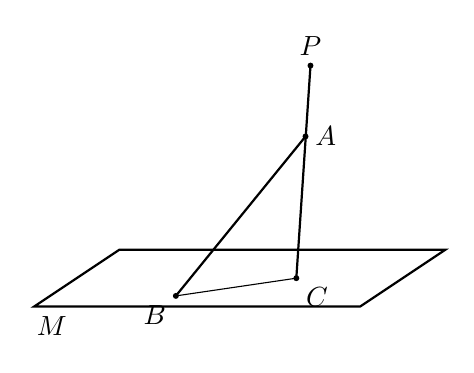
\begin{tikzpicture}[scale=0.9]
  % 地平面 M
  \draw[thick] (0,0) -- (4.6,0) -- (5.8,0.8) -- (1.2,0.8) -- cycle;
  \node[below] at (0.25,0) {$M$};
  % 电柱 PC：C 为柱脚，P 为柱顶，A 在 PC 上
  \draw[thick] (3.7,0.4) -- (3.9,3.4);
  \fill (3.9,3.4) circle (1.2pt) node[above] {$P$};
  \coordinate (A) at (3.83,2.4);
  \fill (A) circle (1.2pt) node[right] {$A$};
  \coordinate (C) at (3.7,0.4);
  \fill (C) circle (1.2pt) node[below right] {$C$};
  % 拉线 AB 与地面段 BC
  \draw[thick] (A) -- (2.0,0.15);
  \draw[thin] (C) -- (2.0,0.15);
  \fill (2.0,0.15) circle (1.2pt) node[below left] {$B$};
\end{tikzpicture}
\end{center}
\nopagebreak[4]
（5） 求出 $A(-3,3)$、$B(0,-1)$、$C(1,0)$ 三点中每两点间的距离，并指出以这三点为顶点的三角形 $ABC$ 是什么样的三角形。

\begin{gktip}
原源 PDF 第 1 页附有坐标系与三点示意图（原卷题注「第一，5题附图」）；LaTeX 版按源图重绘。
\end{gktip}
\nopagebreak[4]
\begin{center}% 1977 年辽宁卷第一题(5)：A(-3,3)、B(0,-1)、C(1,0) 三点与三角形 ABC（按源卷第 1 页「第一，5题附图」布局）
\begin{tikzpicture}[scale=0.72,>=stealth]
  \draw[->] (-4.2,0)--(5.4,0) node[below] {$x$};
  \draw[->] (0,-1.8)--(0,3.9) node[left] {$y$};
  \node[below left] at (0,0) {$O$};
  \draw[thin] (-3,0.07)--(-3,-0.07);
  \draw[thin] (1,0.07)--(1,-0.07);
  \draw[thin] (0.07,-1)--(-0.07,-1);
  \draw[thin] (0.07,3)--(-0.07,3);
  \draw[thick] (-3,3)--(0,-1)--(1,0)--cycle;
  \fill (-3,3) circle (1.2pt) node[left=2pt] {$A(-3,3)$};
  \fill (0,-1) circle (1.2pt) node[below right] {$B(0,-1)$};
  \fill (1,0) circle (1.2pt) node[above right] {$C(1,0)$};
\end{tikzpicture}
\end{center}
\nopagebreak[4]
\end{question}
\begin{question}
\gkti{2}判别二次函数 $y=x^2-4x+3$ 有最大值还是有最小值？并把它求出来；写出这个函数图象的顶点坐标，用描点法画出这个函数的图象。（画出草图即可）

\end{question}
\begin{question}
\gkti{3}制造某种产品，计划经过两年使成本降低 36\%，问平均每年应降低百分之几？

\end{question}
\begin{question}
\gkti{4}在 $\triangle ABC$ 中，已知 $\operatorname{Cos}A=\dfrac5{13}$，$\operatorname{Cos}B=\dfrac35$，求 $\operatorname{Cos}C$ 的值。

\end{question}
\begin{question}
\gkti{5}求证：两条对角线相等的梯形是等腰梯形（画出图形，写出：已知、求证、证明）。

\end{question}
\begin{question}
\gkti{6}$\alpha$ 是多少度时，方程 $2x^2+2\sqrt2\,x+\operatorname{tg}\alpha=0$ 有两个相等的实数根？（$0^\circ\le\alpha<360^\circ$）

\Needspace{0.4\textheight}
\end{question}
\begin{question}
\gkti{7}如图，我海军某舰艇在 $A$ 处测得入侵敌舰在方位角为 $45^\circ$、距离为 10 海里的 $C$ 处，并正沿方位角为 $105^\circ$ 的方向以每小时 9 海里的速度逃跑，我舰艇立即以每小时 21 海里的速度沿直线前去追捕，问我舰艇应沿多大的方位角和需用多少小时才能在某处 $B$ 追上敌舰？

（已知：$\operatorname{Sin}21^\circ47'=\dfrac{3\sqrt3}{14}$，$\operatorname{Sin}38^\circ13'=\dfrac{5\sqrt3}{14}$。这两个数据可根据解题需要取用。）

\begin{gktip}
原源 PDF 第 4 页附有 A、C 两处北向箭头与追击路线示意图（原卷题注「第七题附图」）；LaTeX 版按源图重绘。
\end{gktip}
\nopagebreak[4]
\begin{center}% 1977 年辽宁卷第七题：A 处测得敌舰 C（方位角 45°、距离 10 海里），
% 敌舰沿方位角 105° 方向逃跑，我舰沿海面直线 AB 追至 B 追上
% （按源卷第 4 页「第七题附图」布局：A、C 处各画北向箭头，A 处标 45°，C 处标 105°）
\begin{tikzpicture}[scale=0.62,>=stealth]
  \coordinate (A) at (0,0);
  \coordinate (C) at (3.5,3.5);
  \coordinate (B) at (9.3,1.95);
  \draw[->] (A) -- (0,2.2) node[draw=none,above] {北};
  \draw[->] (C) -- (3.5,5.2) node[draw=none,above] {北};
  \draw[thick] (A)--(B)--(C)--cycle;
  \draw[thin] ([shift={(A)}]45:0.8) arc[start angle=45,end angle=90,radius=0.8];
  \node at (0.40,0.97) {$45^\circ$};
  \draw[thin] ([shift={(C)}]-15:0.7) arc[start angle=-15,end angle=90,radius=0.7];
  \node at (4.25,4.08) {$105^\circ$};
  \fill (A) circle (1.2pt) node[below left] {$A$};
  \fill (C) circle (1.2pt) node[above left] {$C$};
  \fill (B) circle (1.2pt) node[right] {$B$};
\end{tikzpicture}
\end{center}
\nopagebreak[4]
\begin{gktip}
\textbf{参考题}
\end{gktip}

\textbf{参考题 1．} 某生产队要建造一个已知体积为 $V$ 的有盖圆柱形氨水池，问这个氨水池的高 $h$ 和底面半径 $r$ 取多大时，用料最省？

\begin{gktip}
原源 PDF 第 7 页附有氨水池（圆柱）高 $h$ 与底面半径 $r$ 示意图；LaTeX 版按源图重绘。
\end{gktip}
\nopagebreak[4]
\begin{center}% 1977 年辽宁卷参考题一：有盖圆柱形氨水池，标高 h 与底面半径 r（按源卷第 7 页布局）
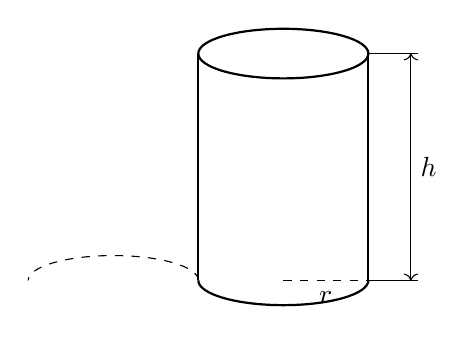
\begin{tikzpicture}[scale=0.9]
  \draw[thick] (1.2,3.2) ellipse (1.2 and 0.35);
  \draw[thick] (0,3.2)--(0,0);
  \draw[thick] (2.4,3.2)--(2.4,0);
  \draw[thick] (0,0) arc[x radius=1.2,y radius=0.35,start angle=180,end angle=360];
  \draw[dashed] (0,0) arc[x radius=1.2,y radius=0.35,start angle=0,end angle=180];
  % 底面半径 r（中心到右缘，虚线）
  \draw[dashed] (1.2,0)--(2.4,0);
  \node[draw=none,below] at (1.8,-0.02) {$r$};
  % 高 h（右侧尺寸线）
  \draw[thin] (2.4,0) -- (3.1,0);
  \draw[thin] (2.4,3.2) -- (3.1,3.2);
  \draw[<->] (3.0,0)--(3.0,3.2) node[midway,right] {$h$};
\end{tikzpicture}
\end{center}
\nopagebreak[4]
\textbf{参考题 2．} 求 $y=\operatorname{Sin}x$（$x$ 在 $[0,\pi]$ 上）与 $x$ 轴所围成的图形的面积。
\nopagebreak[4]
\begin{center}% 1977 年辽宁卷参考题二：y=Sinx 在 [0,π] 与 x 轴之间的阴影区域（按源卷第 7 页「参考题二附图」布局）
% 源卷图内标注印作「y=Sinπ」，系排印之误，重绘图按 y=Sinx 标注
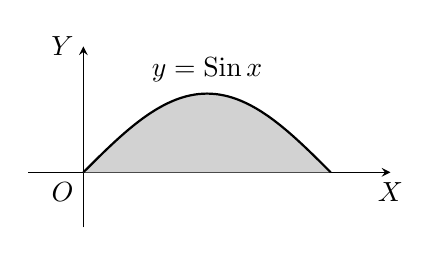
\begin{tikzpicture}[scale=1.0,>=stealth]
  \draw[->] (-0.7,0)--(3.9,0) node[below] {$X$};
  \draw[->] (0,-0.7)--(0,1.6) node[left] {$Y$};
  \node[below left] at (0,0) {$O$};
  \fill[gray!35] (0,0) -- plot[domain=0:3.1416,smooth] (\x,{sin(\x r)}) -- cycle;
  \draw[thick,domain=0:3.1416,smooth] plot (\x,{sin(\x r)});
  \node[draw=none,above] at (1.57,1.02) {$y=\operatorname{Sin}x$};
\end{tikzpicture}
\end{center}
\nopagebreak[4]
\begin{gktip}
原源 PDF 第 7 页附有 $y=\operatorname{Sin}x$ 在 $[0,\pi]$ 上与 $x$ 轴之间的阴影区域示意图（源卷图内标注印作「y=Sinπ」，系排印之误）；LaTeX 版按源图重绘并按 $y=\operatorname{Sin}x$ 标注。
\end{gktip}


\end{question}
\end{document}
